\section{Motivation}
\label{sec:motivation}

Even though batch, interactive, and streaming applications all care about performance, their notions of performance are different.
For instance, while the average completion time can sufficiently capture the performance of a throughout-sensitive batch-job queue (\batchq) \cite{tetris}, interactive sessions and streaming applications form latency-sensitive queues (\burstq): each \burstq is a sequence of small jobs following an ON-OFF pattern. 
For these jobs \cite{spark-streaming}, individual completion times or latencies are far more important than the average completion time or the throughput of the \burstq.

%\begin{figure}[!t]
%	\centering
%	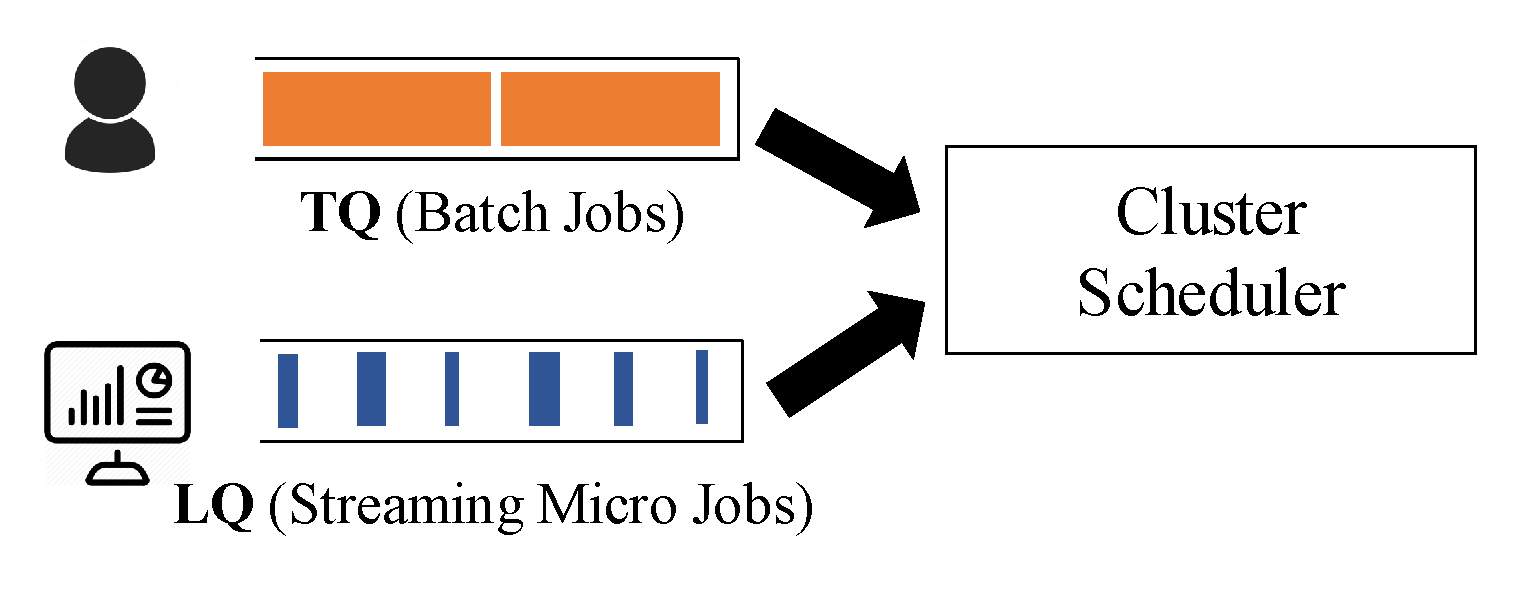
\includegraphics[width=0.8\columnwidth]{fig/queues.pdf}%
%	\caption{Users and automated processes submit throughput-sensitive (TQ) and latency-sensitive (LQ) to the same cluster.}
%	\label{fig:queues}
%	\vspace{-0.1in}
%\end{figure} 

Indeed, existing ``fair'' schedulers are inherently unfair to \burstq jobs: when \burstq jobs are present (ON state), they must share the resources equally with \batchq jobs, but when they are absent (OFF state), batch jobs get all the resources. 
In the long run, {\batchq}s receive more resources than their fair shares because today's schedulers such as Dominant Resource Fairness~\cite{drf} make \emph{instantaneous} decisions.

%Therefore, we ponder a fundamental question: \emph{can we enable latency-sensitive {\burstq}s and throughput-sensitive {\batchq}s to coexist, where {\burstq}s are permitted short-term resource bursts while ensuring long-term fairness between the two, as well as maximizing {\burstq}s served with resource guarantees?}

Clearly, it is impossible to achieve the best response time for \burstq jobs under \emph{instantaneous} fairness. 
In other words, there is a hard tradeoff between providing instantaneous fairness for {\batchq}s and minimizing the response time of {\burstq}s. 
However, instantaneous fairness is not necessary for {\batchq}s because average-completion time over a relatively long time horizon is their most important metric.
This sheds light on the following question: \emph{how well can we simultaneously accommodate multiple classes of workloads with performance guarantees, in particular, isolation protection for {\batchq}s in terms of long-term fairness and low response times for {\burstq}s}? 


%In this work, we explore opportunities and challenges in achieving three desired properties: (i) allowing {\burstq}s to enjoy short-term high resource usage during their ON periods to minimize \emph{individual} job response times; (ii) maintaining the same \emph{long-term} fairness as existing ``fair'' allocation policies by preventing arbitrarily large bursts; and (iii) maximizing system utilization and {\burstq}s served with resource guarantees.

This work serves as our first step in answering the question by designing \name: the first multi-resource scheduler that achieves both isolation protection for {\batchq}s and response time guarantees for {\burstq}s in a strategyproof way. 
%It is simple to implement and provides significant performance improvements even in the presence of uncertainties. 
The key idea is ``bounded'' priority for {\burstq}s: as long as the burst is not too large to hurt the long-term fair share of {\batchq}s and other {\burstq}s, they are given higher priority so jobs can be completed as quickly as possible. %However, there are several challenges. There is a fundamental tradeoff between ``hard'' resource guarantee to {\burstq}s and isolation protection for {\batchq}s. In addition, naive admission control may result in very few {\burstq}s admitted.